\chapter{Performance Benchmarks}

\section{Single-Node Benchmarks}

\subsection{Hardware Description}

\begin{table}[!h]
  \centering
\begin{tabular}{l| c c c c c}
    \hline
  Hardware & Cores/SP & Memory  [GB] & Theoretical Bandwidth [GB/s] & Backend & Notes\\
    \hline \hline
  2x Xeon E5-2630 v3& 2x 8 & 128 & 2x 59   & OpenMP(Host) & NUMA
  \\ \hline  
  2x Xeon E5-2630 v3& 2x 8 & 128 & 2x 59   & MPI(Host)    & NUMA\\ \hline
  Core i7 4770K     &   4  & 32  & 25.6    & OpenMP(Host) & UMA\\ \hline
  MIC/Xeon Phi 5110 &   60 & 8   &  320    & OpenMP(MIC)  & ECC\\ \hline
  K40               &  2880& 12  &  288    & CUDA/OpenCL  & ECC\\ \hline
  GTX970            &  1664& 4   &  192    & CUDA/OpenCL  & no ECC\\ \hline
  FirePro (FP) W9100&  2816& 16  &  320    & OpenCL       & no ECC\\ \hline
\end{tabular}
\caption{Hardware configurations}
\end{table}

The performance values are obtained with the "benchmark" tool from the PARALUTION package. The tool is compiled on various systems, no code modification is applied. The operating system (OS) for all hardware configurations is Linux. All tests are performed in double precision.

The hardware specifications are obtained from
Intel
\footnote{Intel E5-2630 v3: http://ark.intel.com/products/83356/Intel-Xeon-Processor-E5-2630-v3-20M-Cache-2\_40-GHz}
\footnote{Intel Core i7 4770K: http://ark.intel.com/products/75123/}
\footnote{Intel Xeon Phi 5110P: http://ark.intel.com/products/71992/Intel-Xeon-Phi-Coprocessor-5110P-8GB-1\_053-GHz-60-core},
AMD
\footnote{AMD FirePro W9100: www.amd.com/en-us/products/graphics/workstation/firepro-3d/9100}
and
NVIDIA
\footnote{NVIDIA GTX970: http://www.geforce.com/hardware/desktop-gpus/geforce-gtx-970/specifications}
\footnote{NVIDIA K40: http://www.nvidia.com/object/tesla-servers.html}
websites.

The configuration is:
\begin{itemize}
  \item PARALUTION - version M1.2.0
 \item Host/OpenMP -- the number of threads is equal to the number of real cores (no HT), gcc versions 4.8.5
 \item CUDA -- CUDA version 7.5
 \item OpenCL -- NVIDIA OpenCL version 1.2 (comes with CUDA 7.5); AMD OpenCL version 2.0
 \item MIC/OpenMP -- for the Xeon Phi, the number of threads for the OpenMP section is not set (the default configuration is used), icc version 13.1
\end{itemize}


\subsection{BLAS1 and SpMV}

The vector-vector routines (BLAS1) are performed with size 4,000,000 -- Figure~\ref{perf-BLAS1}.

\begin{itemize}
    \item ScaleAdd is $x = \alpha x + y$, where $x,y \in \mathbb{R}^n$ and $\alpha \in \mathbb{R}$
    \item Dot product is $\alpha = \sum_{i=0}^{n} x_i y_i$, where $x,y \in \mathbb{R}^n$ and $\alpha \in \mathbb{R}$
    \item Reduce is $\alpha = \sum_{i=0}^n x_i$, where $x \in \mathbb{R}^n$ and $\alpha \in \mathbb{R}$
    \item $L^2$ Norm is $\alpha = \sqrt{\sum_{i=0}^n x_i^2}$, where $x \in \mathbb{R}^n$ and $\alpha \in \mathbb{R}$
  \end{itemize}

The backends for all vector-vector routines are CUDA for NVIDIA GPU; OpenCL for AMD GPU; OpenMP for Host/MIC.

\begin{figure}[h!]
\centering
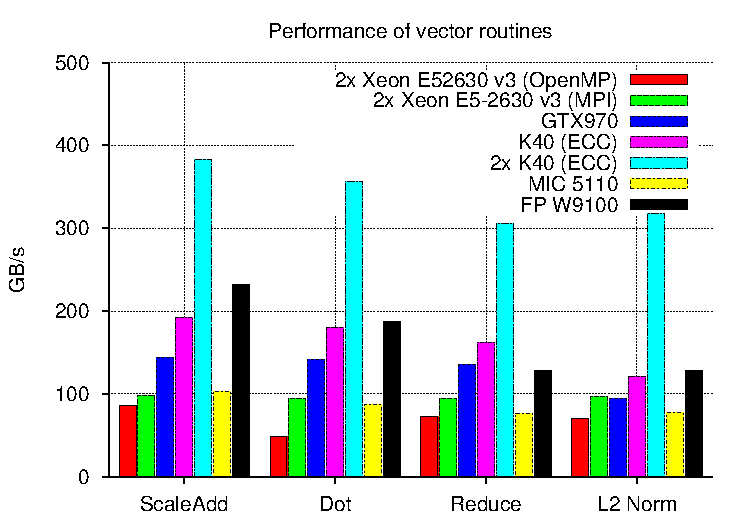
\includegraphics[width=0.75\textwidth]{./fig/perf/BLAS1.pdf}
\caption{BLAS1 routines}
\label{perf-BLAS1}
\end{figure}

The SpMV (sparse matrix-vector multiplication) is computed using a 2D Laplace (structured grid, finite difference) matrix on a grid with 2,000 $\times$ 2,000 = 4,000,000 DoFs -- Figure~\ref{perf-BLAS2}.

All routines are executed 100 times and the average time (in ms resolution) is taken.

\begin{figure}[h!]
\centering
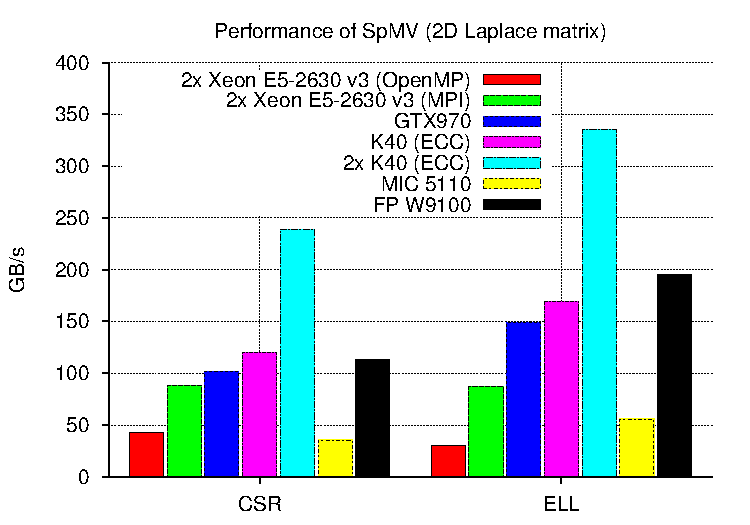
\includegraphics[width=0.75\textwidth]{./fig/perf/BLAS2.pdf}
\caption{SpMV}
\label{perf-BLAS2}
\end{figure}

\subsection{CG Solver}

Furthermore, a non-preconditioned CG has been performed on a Laplace matrix resulting from a Finite
Difference discretization of the unit square with 4.000.000 unknowns (as for the SpMV tests) on all
listed architectures -- Figure~\ref{perf-CG-CPU} and Figure~\ref{perf-CG-GPU}. 
The right-hand side is set to one, initial guess to zero. A relative tolerance of 1e-6 based on L2 norm is used.

\begin{figure}[h!]
\centering
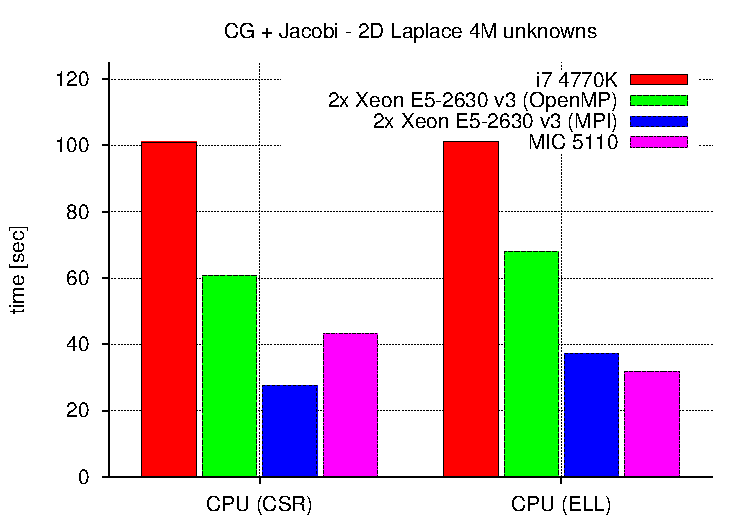
\includegraphics[width=0.75\textwidth]{./fig/perf/CG_CPU.pdf}
\caption{CG CPU Performance}
\label{perf-CG-CPU}
\end{figure}

\begin{figure}[h!]
\centering
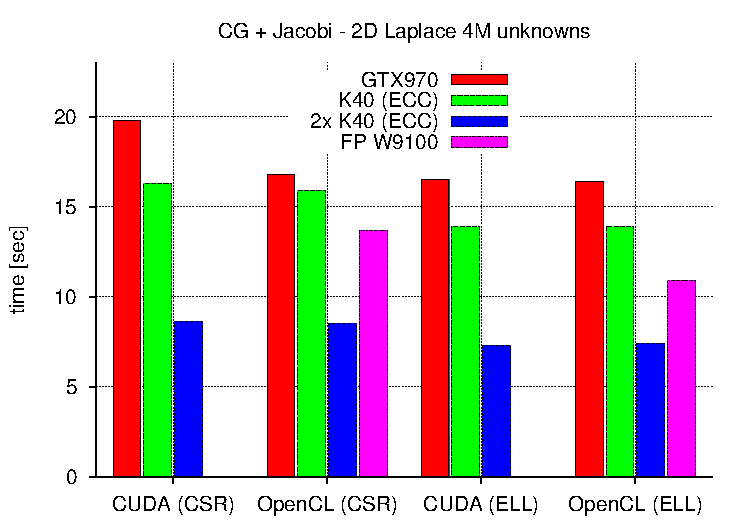
\includegraphics[width=0.75\textwidth]{./fig/perf/CG_GPU.pdf}
\caption{CG GPU Performance}
\label{perf-CG-GPU}
\end{figure}

